Warum wird mit der Entwicklung einer Softwarearchitektur am Anfang eines Projekts begonnen?

\section*{Antwort}
Die Einbeziehung von Software-Architekten direkt zu Beginn eines Projektes (etwa bei der Klärung der Geschäftsanforderungen) erlaubt Einschätzungen bzgl. \textbf{Machbarkeit} und \textbf{Aufwand} (als ``Grundlage für Überlegungen zur Wirtschaftlichkeit``~\cite[37]{Wed09b}).\\
Beides kann Anforderungen, Entscheidungen und somit den weiteren Verlauf des Projektes maßgeblich beeinflussen, {bspw.} durch Erfahrungen, die ein Architekt in ähnlichen Projekten gesammelt hat\footnote{
    wie Qualitätsanforderungen technische Entscheidungen beeinflussen können, zeigen \textit{Bass, Clements, und Kazman} in~\cite[41]{BCK12}.
}.\\
Den hierbei entstehend auch ein Rückkoppelungseffekt: Die Ideen des Kunden beeinflussen die Ideen des Architekten, die wiederum die Ideen des Kunden beeinflussen können (s. Abbildung~\ref{fig:aic}).\\


\begin{figure}
    \centering
    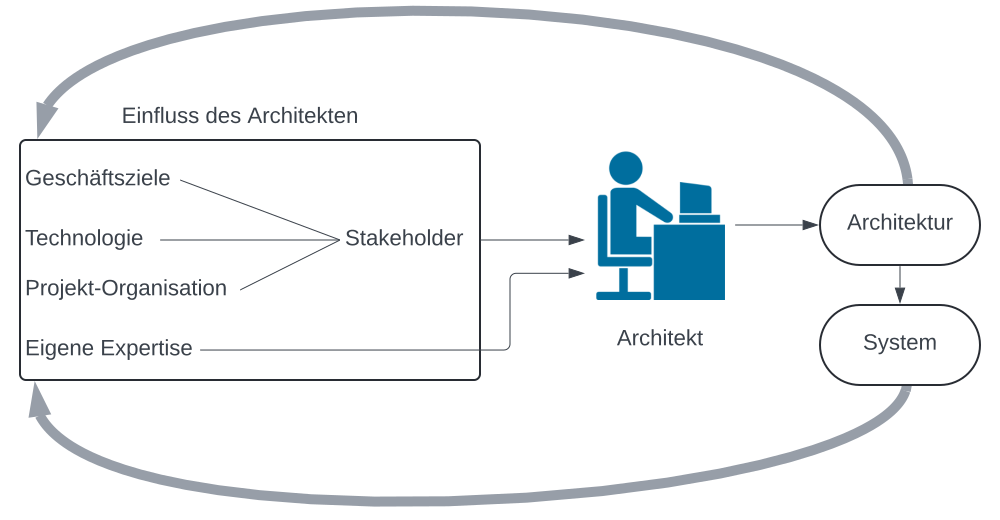
\includegraphics[scale=0.4]{chapters/aufgabe 6/img/aic}
    \caption{Der \textit{Architecture Influence Cycle} nach \textit{Bass, Clements, und Kazman}. Qualitäts-, Geschäfts- und organisatorische Anforderungen beeinflussen die Arbeit des Architekten, die wiederum diese Anforderungen beeinflussen können. Zusätzlich wirken eigene Erfahrungen auf seine Planung ein, die wiederum in ein Folgeprojekt einfließen können.  (Quelle: in Anlehnung an~\cite[58, Figure 3.5]{BCK12})}
    \label{fig:aic}
\end{figure}